\documentclass[11pt]{article}
\usepackage[utf8]{inputenc}
\usepackage{amsmath}
\usepackage{amsthm}
\usepackage{amsfonts}
\usepackage{color}
\usepackage{longtable}
\usepackage{tabu}
\usepackage{tikz}

\definecolor{codegray}{gray}{0.9}
\newcommand{\category}[1]{\textbf{\emph{#1}}}
\newcommand{\code}[1]{
  \begin{align*}
    \texttt{#1}
  \end{align*}
  }
\theoremstyle{definition}
\newtheorem{definition}{Definicija}
\newtheorem{primjer}{Primjer}
\newtheorem{koloral}{Koloral}
\newtheorem{teorem}{Teorem}

\begin{document}
  %%%%%%%%%%%%%%%%%%%%%%%%%%%
  %% Definicija Kategorije %%
  %%%%%%%%%%%%%%%%%%%%%%%%%%%
  \section{Kategorije}
  U ovom poglavlju definiramo kategorije i detaljno raspisujemo nekoliko
  primjera.
  Intuitivno, teorija kategorije proucava "objekte" i preslikavanje izmedu
  njih. To su primitivni objekti u teoriji kategorija koje ne definiramo.
  \begin{definition}
    Kategorija $G$ sastoji se od:
    \begin{itemize}
      \item kolekcije objekata $Obj$
      \item kolekcije strelica $Arw$
      \item pridruzivanja $Arw \xrightarrow{source} Obj$
      \item pridruzivanja $Arw \xrightarrow{target} Obj$
      \item pridruzivanja (identiteta) $Obj \xrightarrow{id} Arw$ takvog da
      za $B \xrightarrow{id} id_B$ vrijedi:
        \begin{equation}
          target(id_B) = source(id_B) = B
        \end{equation}
      \item pridruzivanja (kompozicija) $Arw \times Arw \xrightarrow{\circ}
      Arw$ takvog da za \\ $(f, g) \xrightarrow{\circ} f \circ g$ vrijedi:
        \begin{align}
          source(f) &= target(g) \\
          source(f \circ g) &= source(g) \\
          target(f \circ g) &= target(f)
        \end{align}
    \end{itemize}
    Pridruzivanja identiteta ($id$) i kompozicija ($\circ$) moraju
    zadovoljavati:
    \begin{itemize}
      \item svojstvo identiteta: za svaku strelicu $A \xrightarrow{f} B$ vrijedi:
        \begin{align}
          id_B \circ f = f = f \circ id_A
        \end{align}
      \item svojstvo asocijativnost: za sve strelice $A \xrightarrow{f} B
      \xrightarrow{g} C \xrightarrow{h} D$ vrijedi:
        \begin{align} \label{def:kat_assoc}
          (h \circ g) \circ f = h \circ (g \circ f)
        \end{align}
    \end{itemize}
  \end{definition}
  Kada zelimo posebno naglasiti kojoj kategoriji pripadaju strelice i objekti
  onda cemo umjesto $Obj$ i $Arw$ pisati $Obj_G$ i $Arw_G$.
  Za $A, B \in Obj_G$ skup svih strelica sa $A$ u $B$ oznacavamo sa
  \category{G}$[A, B]$.
  Sada cemo detaljno raspisati nekoliko primjera kategorija.

  %%%%%%%%%%%%%%%%%%%%
  %% Mon Kategorija %%
  %%%%%%%%%%%%%%%%%%%%
  \begin{primjer}
    \textbf{Monoid} je uredena trojka $(M, \cdot_M, 1_M)$ gdje je $M$ skup, $1_M
    \in M$, $\cdot_M$ binarna operacija na $M$ za koju vrijedi da za svaki $a, b, c \in M$:
    \begin{equation*}
      (a \cdot_M b) \cdot_M c = a \cdot_M (b \cdot_M c)
    \end{equation*}
    \begin{equation*}
      1_M \cdot_M a = a = a \cdot_M 1_M
    \end{equation*}
    Neutralni element $1_M$ i binarnu operaciju $\cdot_M$ cemo uglavnom pisati
    kao $1$ i $\cdot$ osim ako nece biti jasno iz konteksta na kojem monoidu
    su defnirani.
    Kada monoid promatramo kao kategoriju tada su objekti elementi skupa M, a
    za dva monoida $M, N$ definiramo strelicu $M \xrightarrow{\delta} N$ kao
    funkciju za koju vrijedi da za svaki $a, b \in M$ vrijedi:
    \begin{equation*}
      \delta(a \cdot b) = \delta(a) \cdot \delta(b)
    \end{equation*}
    \begin{equation*}
      \delta(1) = 1
    \end{equation*}
    i zovemo ju \textbf{morfizam}.
    Pokazimo da je kompozicija dva morfizma morfizam.
    Neka su $a, b \in Obj_M$ i $M \xrightarrow{f} N \xrightarrow{g} P$, tada vrijedi:
    \begin{equation*}
      (g \circ f)(a \cdot b) = g(f(a \cdot b)) = g(f(a) \cdot f(b)) = g(f(a))
      \cdot g(f(b)) = (g \circ f)(a) \cdot (g \cdot f)(b)
    \end{equation*}
    Za monoid $M$ definiramo identitetu $id_M$ kao standardnu funkciju
    identiteta, tj. za svaki $a \in Obj_M$ vrijedi:
    \begin{equation*}
      id_M(a) = a
    \end{equation*}
    Pokazimo sada da tako definiran strelice na monoidu zadovoljavaju
    svojstvo identiteta i asocijativnosti (\ref{def:kat_assoc}) za kategorije.
    Neka je $a \in Obj_M$ i $M \xrightarrow{f} N$, tada vrijedi:
    \begin{equation*}
      (id_N \circ f)(a) = id_N(f(a)) = f(a) = f(id_M(a)) = (f \circ id_M)(a)
    \end{equation*}
    te je svojstvo identiteta zadovoljeno.
    Neka su $M, N, P, R$ monoidi, $M \xrightarrow{f} N \xrightarrow{g} P \xrightarrow{h} R$
    i $a \in Obj_M$, tada vrijedi:
    \begin{equation*}
      ((h \circ g) \circ f)(a) = h(g(f(a))) = (h \circ (g \circ f))(a)
    \end{equation*}
    zbog asocijativnosti kompozicije funkcija te monoide mozemo promatrati kao
    kategorije. Kategoriju monoida oznacavamo sa \category{Mon}.
  \end{primjer}

  %%%%%%%%%%%%%%%%%%%%
  %% Pos Kategorija %%
  %%%%%%%%%%%%%%%%%%%%
  \begin{primjer}
    Neka je $S$ skup i $\leq_S \subseteq S \times S$ relacija na $S$. Uredeni par $(S,
    \leq_S)$ zovemo \textbf{parcijalno uredeni skup} ako za svaki $a, b, c \in S$
    vrijedi:
    \begin{itemize}
      \item $a \leq_S a$ (refleksivnost)
      \item ako $a \leq_S b$ i $b \leq_S a$ tada $a = b$ (anti-simetricnost)
      \item ako $a \leq_S b$ i $b \leq_S c$ tada $a \leq_S c$ (tranzitivnost)
    \end{itemize}
    Radi kraceg zapisa pisati cemo samo $\leq$ umjesto $\leq_S$ i
  govoriti o parcijalno uredenom skupu $S$ gdje je implicitno definirna
  binarna relacija $\leq$.
  Neka su $S, R$ dva parcijalno uredena skupa i neka je $R \xrightarrow{f} S$
  preslikavanje za koje vrijedi da za svaki $a, b \in S$ vrijedi:
  \begin{equation*}
    a \leq b \implies f(a) \leq f(b)
  \end{equation*}
  Tada kazemo da je $f$ \textbf{monotono preslikavanje}.
  Pokazimo da su monotona preslikavanja zatvorena na kompoziciju.
  Neka su $S \xrightarrow{f} R \xrightarrow{g} Q$ monotona preslikavanja i $a,
  b \in S$ takva da $a \leq b$. Tada vrijedi:
  \begin{equation*}
    a \leq b \implies f(a) \leq f(b) \implies g(f(a)) \leq g(f(b))
  \end{equation*}
  tj.
  \begin{equation*}
    a \leq b \implies (g \circ f)(a) \leq (g \circ f)(b)
  \end{equation*}
  Identiteta na parcijalnu uredenom skupu $S$ je definirana kao standardna
  funkcijska identiteta. Kao i u prethodnom primjeru pokaze se da vrijedi:
  \begin{equation*}
    (id_R) \circ f = f = f \circ id_S
  \end{equation*}
  \begin{equation*}
    (h \circ g) \circ f = h \circ (g \circ f)
  \end{equation*}
  pa mozemo govoriti u kategoriji \category{Pos} gdje su objekti parcijalno
  uredeni skupovi a strelice monotona preslikavanja.
  \end{primjer}
  %%%%%%%%%%%%%%%%%%%%%
  %% Hask Kategorija %%
  %%%%%%%%%%%%%%%%%%%%%
  \begin{primjer} \category{Hask} je kategorija Haskellovih tipova i funkcija. U
  \category{Hask} kategoriji objekti su Haskellovi tipovi koje oznacavamo velikim
  slovima:
    \code{A, B, C, ...}
  Strelice u \category{Hask}-u su Haskellove funkcije koje oznacavamo malim
  slovima:
    \code{f, g, h, ...}
  Strelicu $A \xrightarrow{f} B$ u \category{Hask}-u zapisujemo:
    \code{f :: A -> B}
  Funkcije
    \code{
      f :: A -> B, g :: A -> B
      }
  su jednake ako za svaki \texttt{x} vrijedi:
    \code{ f x = g x }
  Kompoziciju ($A \xrightarrow{f \circ g} C$) zapisujemo:
    \code{(f.g) :: A -> C}
    i definiramo kao standardnu funkcijsku kompoziciju, tj.:
    \code{(f.g) x = f (g x)}
  pa se lako pokaze da vrijedi svojstvo asocijativnosti.
  Identiteta je u \category{Hask}-u dana funkcijom:
    \code{ id x = x }
  te se lako vidi da vrijedi:
    \code{ id.f = f = id.f }
  \end{primjer}

  %%%%%%%%%%%%%%%%%%%%%%%%%%%%%%%%%%%%%%%%%%%%%%%%%%%%%%%
  %% Kategorija gdje strelica nije standardna funkcija %%
  %%%%%%%%%%%%%%%%%%%%%%%%%%%%%%%%%%%%%%%%%%%%%%%%%%%%%%%
  \begin{primjer}
    Pokazimo sada primjer neke kategorije $G$ gdje su objekti konacni skupovi,
    a strelica izmedu objekata ne mora biti uobicajena funkcija.
    Neka su $A, B$ konacni skupovi, strelica $A \xrightarrow{f} B$ je
    proizvoljna funkcija:
    \begin{equation*}
      f:A \times B \rightarrow \mathbb{R}
    \end{equation*}
    Za strelice $A \xrightarrow{f} B \xrightarrow{g} C$ definiramo:
    \begin{equation*}
      g \circ f:A \times C \rightarrow \mathbb{R}
    \end{equation*}
    sa
    \begin{equation*}
      (g \circ f)(a, c) = \sum\{f(a, y)g(y,c) | y \in B\}
    \end{equation*}
    Lako je vidjeti da je to kategorija.  \end{primjer}

  %%%%%%%%%%%%%%%%%%%%%%%
  %% Dualna kategorija %%
  %%%%%%%%%%%%%%%%%%%%%%%
  \begin{primjer}
    Neka je $G$ neka kategorija. Tada definiramo kategoriju $G^{op}$ koja ima
    iste objekte kao i $G$, a za svaku strelicu u $G$, $A \xrightarrow{f} B$
    definirana je dualna strelicu u $G^{op}$, $B \xrightarrow{f^{op}} A$.
    Za strelice $A \xrightarrow{f} B \xrightarrow{g} C$ kompozicija strelica
    u $G^{op}$ definirana je sa:
    \begin{equation*}
      f^{op} \circ^{op} g^{op} = (g \circ f)^{op}
    \end{equation*}
    Pokazimo da tako definirana struktura $G^{op}$ zadovoljava svojstvo
    asocijativnosti i identiteta, tj. da je tako zadana struktura stvarno
    kategorija.
    Neka su $A \xrightarrow{f} B \xrightarrow{g} C \xrightarrow{h} D$, tada je:
    \begin{equation*}
      id^{op}_B \circ^{op} f^{op} = (id_B \circ f)^{op} = (f \circ id_A)^{op} =
      f^{op}
    \end{equation*}
    i
    \begin{align*}
      (h^{op} \circ^{op} g^{op}) \circ^{op} f^{op} &= (h \circ g)^{op} \circ^{op} f^{op}\\
      &= ((h \circ g) \circ f)^{op}\\
      &= (h \circ (g \circ f))^{op}\\
      &= h^{op} \circ^{op} (g \circ f)^{op}\\
      &= h^{op} \circ^{op} (g^{op} \circ^{op} f^{op})
    \end{align*}
    Pa je $G^{op}$ kategorija.
  \end{primjer}
  %%%%%%%%%%%%%%%%%%%%%%%%
  %% Tablica Kategorija %%
  %%%%%%%%%%%%%%%%%%%%%%%%
  Navedimo sada primjere jos nekih kategorija koje cemo kasnije definirati.
  \begin{center}
  \begin{longtabu}{l l l}  \vspace{1em}
    Kategorija & Objekti & Strelice \\
    \category{Set} & skupovi & totalne funkcije \\
    \category{RelA} & skupovi & binarne relacije \\
    \category{Pfn} & skupovi & parcijalne funkcije \\
    \category{Mon} & monoid & morfizmi \\
    \category{Sgp} & polugrupe & morfizmi \\
    \category{CMon} & komutativni monoidi & morfizmi \\
    \category{Grp} & grupe & morfizmi \\
    \category{AGrp} & abelove grupe & morfizmi \\
    \category{Rng} & prstenovi & morfizmi \\
    \category{Pos} & parcialno uredeni skupovi & monotona preslikavanja \\
    \category{Top} & topoloski prostori & neprekidna preslikavanja \\
    \category{Vec$_K$} & Vektorski prostori nad poljem $K$& linearna preslikavanja \\

    \end{longtabu}
  \end{center}

  %%%%%%%%%%%%%%%%%%%%%%%%
  %%%%%%%%%%%%%%%%%%%%%%%%
  %%%%%%% DIJAGRAM %%%%%%%
  %%%%%%%%%%%%%%%%%%%%%%%%
  %%%%%%%%%%%%%%%%%%%%%%%%

  \section{Dijagram}
  U teoriji kategorija dijagrame koristimo kao reprezentaciju jednadzbi.
  Za kategoriju \category{G} i $A, B \in Obj_G$ vec smo vidjeli da
  preslikavanje $f \in \category{G}[A, B]$ oznacavamo dijagramom
  \begin{align*}
    A \xrightarrow{f} B
  \end{align*}
  Pogledajmo slijedeci dijagram sa tri strelice:
  \begin{center}
    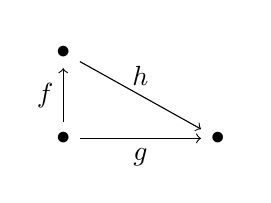
\begin{tikzpicture}[every node/.style={midway}]
      \matrix[column sep={5em,between origins}, row sep={2em}] at (0,0)
      {
        \node(A) {$\bullet$};\\
        \node(B) {$\bullet$}; & \node(C) {$\bullet$}; \\
      };

      \draw[<-] (A) -- (B) node[anchor=east] {$f$};
      \draw[->] (B) -- (C) node[anchor=north]  {$g$};
      \draw[->] (A) -- (C) node[anchor=south] {$h$};
    \end{tikzpicture}
  \end{center}
  Primjetimo da objektima nismo dali imena (zato sto nam za ovaj primjer nije
  bitno), ali to ne znaci da su ta tri objekta jednaka. Ako vrijedi
  \begin{align*}
    g \circ f = h
  \end{align*}
  tada kazemo da dijagram \textbf{komutira}.
  Dijagramom zakon asocijativnosti za $f, g, h$ mozemo prikazati kao:
  \begin{center}
    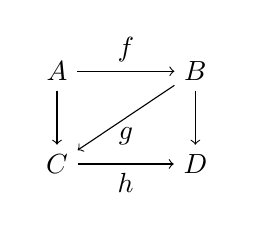
\begin{tikzpicture}[every node/.style={midway}]
      \matrix[column sep={5em,between origins}, row sep={2em}] at (0,0)
      {
        \node(A) {$A$}; & \node(B) {$B$}; \\
        \node(C) {$C$}; & \node(D) {$D$}; \\
      };
      \draw[->] (A) -- (B) node[anchor=south] {$f$};
      \draw[->] (B) -- (C) node[anchor=north] {$g$};
      \draw[->] (C) -- (D) node[anchor=north] {$h$};

      \draw[->] (A) -- (C) node {};
      \draw[->] (B) -- (D) node {};
    \end{tikzpicture}
  \end{center}


  Kao i u mnogim granama matematike u teoriji kategorija ponekad zelimo
  pokazati da su dvije stvari jednake. Rijetko zelimo pokazati da su dva
  objekta jednaka; cesce cemo pokazivati jednakost strelica i za to cemo
  koristiti tehniku zvanu pracenje dijagrama (eng. dijagram chasing).
  Dijagram:

  \begin{center}
    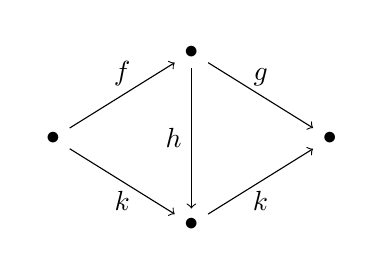
\begin{tikzpicture}[every node/.style={midway}]
      \matrix[column sep={5em,between origins}, row sep={2em}] at (0,0)
      {
        & \node(B) {$\bullet$}; &\\
        \node(A) {$\bullet$}; && \node(C) {$\bullet$}; \\
        & \node(D) {$\bullet$}; & \\
      };
      \draw[->] (A) -- (B) node[anchor=south] {$f$};
      \draw[->] (B) -- (C) node[anchor=south] {$g$};
      \draw[->] (B) -- (D) node[anchor=east] {$h$};
      \draw[->] (A) -- (D) node[anchor=north] {$k$};
      \draw[->] (D) -- (C) node[anchor=north] {$k$};
    \end{tikzpicture}
  \end{center}
  Ima cetiri neimenovana objekta, pet strelica, $f, g, h, k, l$ i pet
  strelica nastalih kompozicijom
  \begin{align*}
    g \circ f, h \circ f, l \circ h \circ f, l \circ h, l \circ k
  \end{align*}
  Primjetimo da neke od tih strelica mogu biti jednake.
  Ovaj dijagram ima tri celije: vanjsku $(f, k, l, g)$, lijevi
  unutarnji trokut $(f, h, k)$ i desni unutarnji trokut $(h, g, l)$.
  Neke od tih celija mogu komutirati:
  \begin{itemize}
      \item lijevi trokut komutira ako vrijedi $h \circ f = k$
      \item desni trokut komutira ako vrijedi $l \circ h = g$
      \item vanjska celija komutira ako vrijedi $g \circ f = l \circ k$
  \end{itemize}
  Pracenje diagrama je proces u kojem pokazemo da neka celija komutira pomocu
  cinjenica da neke druge celije komutiraju i nekih drugih svojstva diagrama

  \begin{primjer} Pokazimo za prijasnji dijagram ako unutarnji trokuti
    komutiraju da tada vanjska celija komutira, tj. da ako vrijedi
    \begin{align*}
      h \circ f = k \qquad  l \circ h = g
    \end{align*}
    trebamo pokazati da vrijedi:
    \begin{align*}
      g \circ f = l \circ k
    \end{align*}
    Algebarski dobivamo:
    \begin{align*}
      g \circ f = (l \circ h) \circ f \overset{(\ref{def:kat_assoc})}{=} l \circ (h \circ f) = l \circ k
    \end{align*}
  \end{primjer}
\end{document}
